\documentclass[professionalfonts]{beamer}
\newif\ifanswers
%\answerstrue % comment out to hide answers
\answersfalse
\usepackage[familydefault,light]{Chivo} 
\usepackage[T1]{fontenc}
\usenavigationsymbolstemplate{}
\usepackage[]{hyperref}
\usepackage{tikz,pgf,pgfarrows,pgfnodes,pgfbaseimage}
\graphicspath{{./Pics/}}
\usetikzlibrary{shapes}
\usepackage{setspace}
\newcommand{\evi}[1]{{\colorbox{yellow!50}{{#1}}}}
\newcommand{\exe}[1]{{\color{black!50}{{#1}}}}
\newcommand{\kw}[1]{{\colorbox{black!30}{\color{white}{#1}}}}
\tikzstyle{nd}=[circle,draw=black,thick,minimum size=.8cm,inner sep=1pt]
\setbeamercovered{transparent}
\usetheme{Singapore}
\tikzstyle{nodo}=[ellipse,draw=black!60,fill=black!10,line width=.7pt,minimum width=.7cm,minimum height=.4cm]
\usecolortheme[named=gray]{structure}
\setbeamercolor{block title}{bg=black!20,fg=black}
\setbeamercolor{block body}{bg=black!10,fg=black}

\ifanswers
\title{Algoritmi Numerici (Parte I)}
\subtitle{[Lezione 2] Numeri Interi $\mathbb{Z}$ e Complemento a Due}
\else
\title{Numerics (Part I)}
\subtitle{[Lecture 2] Integer Numbers $\mathbb{Z}$\\and Two's Complement}
\fi
\date{}
\author{Alessandro Antonucci\\{\tt alessandro.antonucci@supsi.ch}}
%%%%%%%%%%%%%%%%%%%%%%%%%%%%
%\setstretch{1.4}
\begin{document}
    \maketitle
    \frame{
        
        \ifanswers \frametitle{Numeri Naturali ed Addizione}
        \else \frametitle{Natural Numbers and Sum} \fi
        
        \begin{itemize}
            \item \ifanswers Numero = Quantità di elementi in un insieme (cardinalità)
            \else Number = Amount of elements in a set (cardinality) \fi
            \item \ifanswers Es. cardinalità(studenti)=25, cardinalità(docenti)=7
            \else Ex. cardinality(students)=25, cardinality(teachers)=7 \fi
            \item \ifanswers Numeri cardinali detti \evi{naturali} {(\tt unsigned int)}
            \else Cardinal numbers aka \evi{natural}  {(\tt unsigned int)}\fi
            \item \ifanswers Proprietà \evi{ordinale} 
            \else Ordinal property \fi
            $\mathbb{N}=\{0,1,2,\ldots,25,\ldots\}$
            \item \ifanswers Somma? Cardinalità dell'insieme unione 
            \else Cardinality of the union set\fi
            \item \ifanswers Es. cardinalità(studenti $\cup$ docenti) = 32 =: 25 + 7
            \else Ex. cardinality(students $\cup$ teachers) = 32 =: 25 + 7\fi
            \item \ifanswers $\mathbb{N}$ (cardinalità infinita) chiuso rispetto all'addizione
            \else $\mathbb{N}$ (infinite cardinality) closed wrt sums\fi \\
            \ifanswers 
            la somma di due numeri naturali è un numero naturale
            \else
            the sum of two natural numbers is a natural number
            \fi
            \\
            \ifanswers 
            $a \in \mathbb{N},b \in\mathbb{N} \Rightarrow SOMMA(a,b) \in \mathbb{N}$
            \else
            $a \in \mathbb{N},b \in\mathbb{N} \Rightarrow SUM(a,b) \in \mathbb{N}$
            \fi
    \end{itemize}}

\frame{
\ifanswers \frametitle{Numeri Interi e Sottrazione}
\else \frametitle{Integer Numbers and Substraction} \fi

\begin{itemize}
\item \ifanswers Sottrazione = Operazione inversa rispetto all'addizione
\else Subtraction = Inverse operation of sum \fi \\
\ifanswers Dati $b$ e $c$, trova $a$ tale che $b=SOMMA(a,c)$
\else Given $b$ and $c$, find $a$ such that $b=SUM(a,c)$
\fi
\\
\ifanswers 
Es. 32 persone, 25 studenti, quanti insegnanti?\\ $SOTTRAZIONE(32,25)=7$
\else Ex. 32 people, 25 students, how many teachers?\\ $SUBTRACTION(32,25)=7$
\fi
\item
\ifanswers
 $a \in \mathbb{N}, b\in\mathbb{N}$, $SOTTRAZIONE(a,b) \in \mathbb{N} ?$ solo se $a\geq b$!
\else
 $a \in \mathbb{N}, b\in\mathbb{N}$, $SUBTRACTION(a,b) \in \mathbb{N} ?$ only if $a\geq b$!
\fi
\item
\ifanswers
 Se $a<b$: $SOTTRAZIONE(a,b)$ è un numero \evi{negativo}! \\
 $SOTTRAZIONE(a,b):=-SOTTRAZIONE(b,a)$ \\
 $SOTTRAZIONE(5,7):=-SOTTRAZIONE(7,5)=-2$ 
\else
 If $a<b$: $SUBTRACTION(a,b)$ is a \evi{negative} number! \\
$SUBTRACTION(a,b):=-SUBTRACTION(b,a)$ \\
$SUBTRACTION(5,7):=-SUBTRACTION(7,5)=-2$ 
\fi
\item 
\ifanswers
Numeri interi $\mathbb{Z}$ = Numeri naturali $\mathbb{N}$ $\cup$ numeri negativi 
\else
Integer numbers $\mathbb{Z}$ = Natural numbers  $\mathbb{N}$ $\cup$ negative numbers 
\fi
\item 
\ifanswers
 $\mathbb{Z} = \{\ldots,-2,-1,0,+1,+2,\ldots \}$ (cardinalità infinita)
\else
 $\mathbb{Z} = \{\ldots,-2,-1,0,+1,+2,\ldots \}$ (infinite cardinality)
\fi
\end{itemize}}


\frame{
    \ifanswers \frametitle{Memorie a $n$ Bits}
    \else \frametitle{$n$ Bits Memories} \fi
    
    \begin{itemize}
        \item \ifanswers Singolo bit (binary digit) ha due valori/stati ($0$ e $1$)
        \else A single bit (binary digit) has two values/states ($0$ and $1$) \fi 
        \item \ifanswers Memoria a $n$ bits? $2^n$ configurazioni!
        \else $n$ bits memory? $2^n$ configurations!
        \fi
        \item 
        \ifanswers 
        Rappresentare i naturali $\mathbb{N}$? 
        Posizionale in base 2!\\
        Con $n$ bits, rappresento $\{0,1,\ldots,2^n-1\}\subset\mathbb{N}$
        \else
        How to represents natural numbers $\mathbb{N}$? Base 2 positional system!\\
        With $n$ bits, I can represent $\{0,1,\ldots,2^n-1\}\subset\mathbb{N}$
        \fi
        \item 
        \ifanswers 
        Rappresentare gli interi $\mathbb{Z}$?\\
        Un bit per il segno, poi posizionale?\\
        No, non compatto, somma in colonna non funziona!
        \else
        How to represents integer numbers $\mathbb{Z}$? One bit for the signature, the rest positional?\\
        No, redundant and bitwise sum does not work!
        \fi
        \item 
        \ifanswers 
        Soluzione migliore è il \emph{complemento a due}!
        \else
        Better solution is \evi{two's complement}!
        \fi
\end{itemize}}


\frame{\frametitle{\ifanswers Un esempio a 4 bit \else A 4-bits example \fi}
\centering
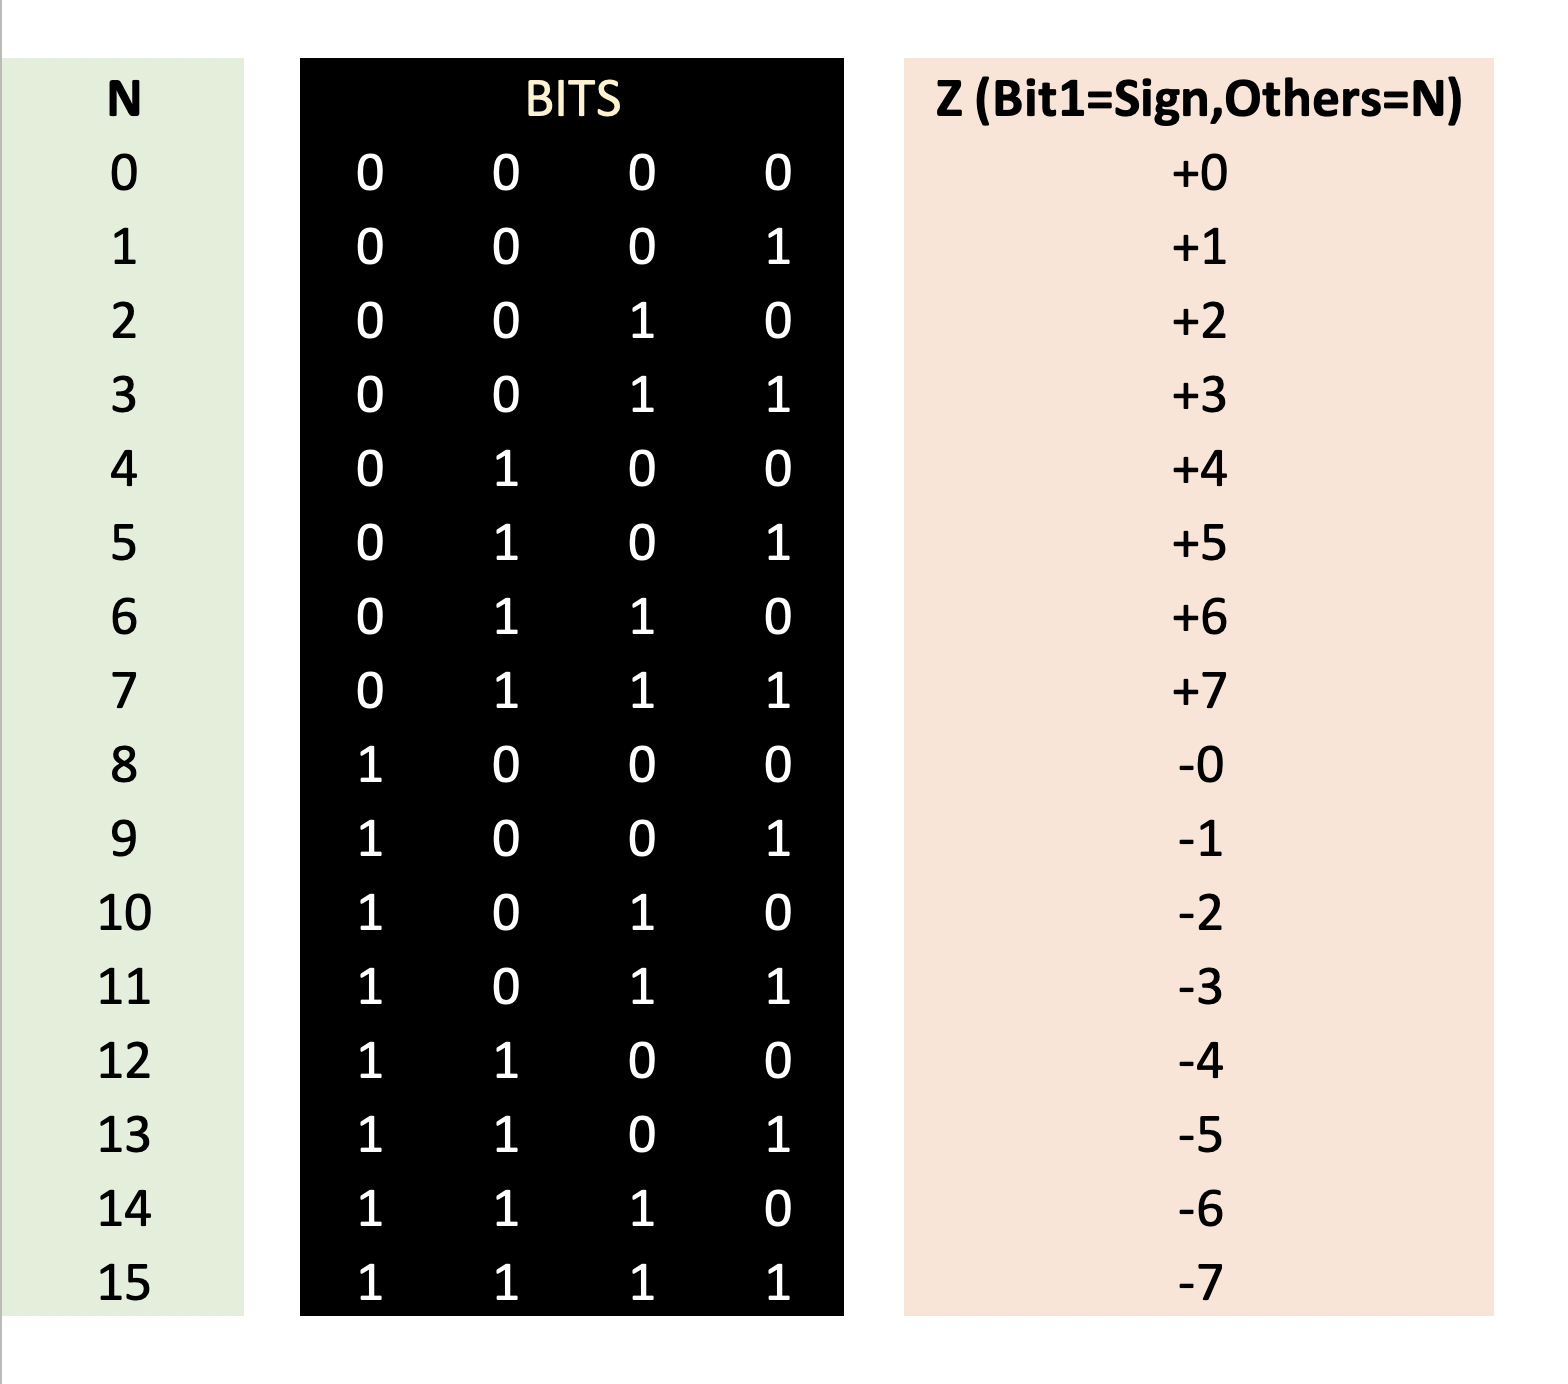
\includegraphics[width=6cm]{z1}\\
\Large
\ifanswers
NO: Facile da capire,\\ma due configurazioni per lo zero\\e somma in colonna non funziona!
\else
NO: Easy to grasp,\\but two configurations for the zero\\and bitwise sum doesn't work!
\fi
}

\frame{\frametitle{\ifanswers Un esempio a 4 bit \else A 4-bits example \fi}
    \centering
    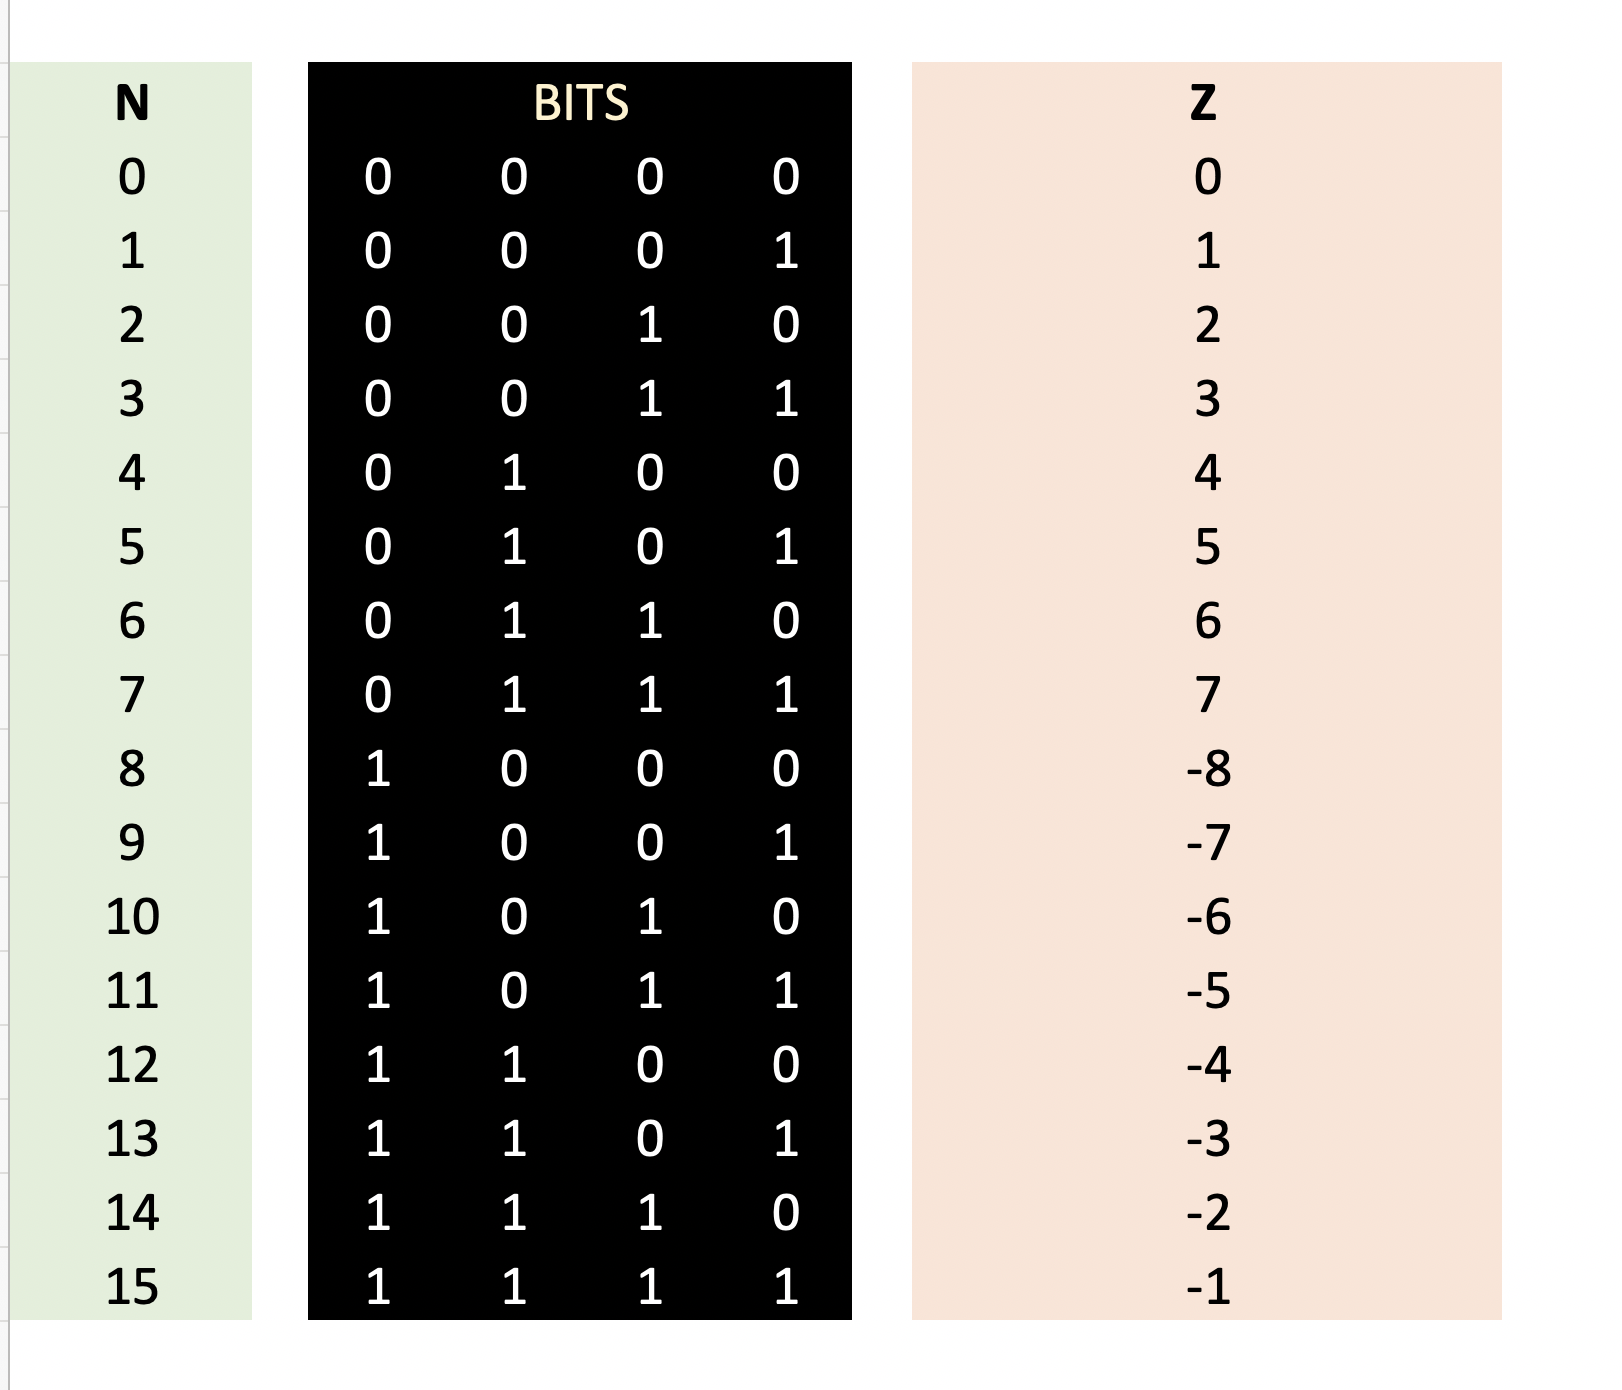
\includegraphics[width=6cm]{z2}\\
\Large
\ifanswers
SI: Pi\`u difficile da capire,\\ma compatto\\e somma in colonna funziona!
\else
YES: Harder to grasp,\\but more compact\\and bitwise sum work!
\fi
}


\frame{\frametitle{\ifanswers Il complemento a 2 \else Two's complement \fi}
\centering
\ifanswers
Linguaggio per rappresentare interi $\mathbb{Z}$ con memorie $n$ bit
\else
Language to represent integers $\mathbb{Z}$ with $n$-bits memories
\fi
\vskip 4mm
\ifanswers
\begin{block}{ALGORITMO DI LETTURA}
\begin{itemize}
\item INPUT = Sequenza di $n$ bits $(b_1,\ldots,b_n)$
\item IF primo bit $=0$
\item ALLORA OUTPUT = HORNER(sequenza)
\item ELSE OUTPUT = - ($2^n$-HORNER(sequenza))
\end{itemize}
\else
\begin{block}{NUMBER READING ALGORITHM}
    \begin{itemize}
        \item INPUT = $n$ bits sequence $(b_1,\ldots,b_n)$
        \item IF first bit $=0$
        \item THEN OUTPUT = HORNER(sequence)
        \item ELSE OUTPUT = - ($2^n$-HORNER(sequence))
    \end{itemize}
\fi
\end{block}

\begin{itemize}
\item 0111$\ldots$1 \ifanswers \`e il pi\`u grande positivo \else biggest positive number \fi
\item 1000$\ldots$0 \ifanswers \`e il pi\`u piccolo negativo \else smallest negative number \fi
\item Range $\{-2^{n-1},-1,0,+1,\ldots,2^{n-1}-1\} \subset \mathbb{Z}$
\end{itemize}

}



\frame{\frametitle{\ifanswers Un alternativa per leggere il complemento a 2 \else An alternative reading strategy\fi}
    \centering
    \ifanswers
    \begin{block}{ALGORITMO DI LETTURA (alternativo)}
        \begin{itemize}
            \item INPUT = Sequenza di $n$ bits $(b_1,\ldots,b_n)$
            \item IF primo bit $=0$
            \item ALLORA OUTPUT = HORNER(sequenza)
            \item ELSE 
            \begin{itemize}
            \item Leggi i bit da dx a sx, ricopiali FINCH\`E non trovi un uno
            \item Quando trovi un uno ricopia anche quello, poi NEGA i bit successivi
            \item Chiama sequenza2 il risultato
            \item OUTPUT = - HORNER(sequenza2)
            \end{itemize}
        \end{itemize}
    \end{block}
    \else
    \begin{block}{READING NUMBER ALGORITHM (alternative)}
        \begin{itemize}
            \item INPUT = $n$ bits sequence $(b_1,\ldots,b_n)$
            \item IF first bit $=0$
            \item THEN OUTPUT = HORNER(sequenza)
            \item ELSE 
            \begin{itemize}
                \item Read bits from right to left
                \item copy them UNTIL you find a one
                \item If you get the one, copy it, and NEGATE all the others
                \item sequence2 is the result
                \item OUTPUT = - HORNER(sequence2)
            \end{itemize}
        \end{itemize}
    \end{block}
    
   
    \fi
    
    \vskip 4mm
    \ifanswers
    \emph{\`E una sottrazione $2^n$-numero fatta direttamente in base 2}
    \else
    \emph{Automatic base-2 subtraction $2^n$-number}
    \fi
    \vskip 4mm
    \ifanswers
    NEGA(0)=1 e NEGA(1)=0
    \else
    NEGATE(0)=1 and NEGATE(1)=0
    \fi
}


\frame{\frametitle{\ifanswers Dal numero ai bit \else From numbers to bits \fi}
\begin{minipage}[t]{8cm}
\ifanswers
Rappresentare $-34$\\col complemento a 2 a 8 bit
\else
8-Bits two's complement of $-34$
\fi
\vskip 4mm
$-34 = -(2^8-x) \Rightarrow x=2^8-34=222$
\vskip 4mm
$-34 \to$ invhorner(222) $\to 1101 1110$
\end{minipage}
\begin{minipage}[t]{2cm}
{\tiny
222 mod 2 = 0\\
111 mod 2 = 1\\
55 mod 2 = 1\\
27 mod 2 = 1\\
13 mod 2 = 1\\
6 mod 2 = 0\\
3 mod 2 = 1\\
1 mod 2 = 1\\
0}
\end{minipage}}

\end{document}
